
%(BEGIN_QUESTION)
% Copyright 2013, Tony R. Kuphaldt, released under the Creative Commons Attribution License (v 1.0)
% This means you may do almost anything with this work of mine, so long as you give me proper credit

Suppose the spring in the main regulator presses upward on the plug with a force of 30 pounds in this pilot-loaded gas pressure regulator system:

$$\includegraphics[width=15.5cm]{i02745x01.eps}$$

Calculate the amount of gas pressure that will be seen at the downstream (exit) port of the main regulator if the pilot is set to output a loading pressure of 4 PSI.  Assume a circular diaphragm in the main regulator with a diameter of 12.75 inches.

\vskip 10pt

\noindent
$P_{out}$ = \underbar{\hskip 50pt} PSI

\vskip 20pt

Also, identify whether each of the mechanisms in this pressure regulation system are {\it force-balance} or {\it motion-balance}:

\vskip 10pt

\noindent
Pilot mechanism = {\it force-balance} or {\it motion-balance}?

\vskip 10pt

\noindent
Main regulator mechanism = {\it force-balance} or {\it motion-balance}?

\vskip 10pt

\underbar{file i02745}
%(END_QUESTION)





%(BEGIN_ANSWER)

I recommend 6 points for the correct calculated pressure, and 2 points each for the type of mechanism balance:

\vskip 10pt

\noindent
$P_{out}$ = \underbar{3.765} PSI
 
\vskip 10pt

\noindent
Pilot mechanism = {\bf force-balance}

\vskip 10pt

\noindent
Main regulator mechanism = {\bf force-balance}


%(END_ANSWER)





%(BEGIN_NOTES)

{\bf This question is intended for exams only and not worksheets!}.

%(END_NOTES)


